\chapter[]{Pubblicità promozione e immagine}
\graphicspath{ {./images/chapter8/} }

La DAF ha propagandato la propria produzione in svariate forme ma soprattutto sui periodici di moda femminile: Vesta, Vendere, Mani di Fata. I prodotti lavorati erano cotone, satin, taffettà, materassè, seta da paracadute, seta pura italiana, georgette. Il marchio di fabbrica era “Sole Onda”, come riportato in figura. 

\begin{figure}[h]
	\centering
		
\includegraphics[width=\textwidth]{marchio_daf.jpg}
	\caption{Marchio di fabbrica della DAF}
	\label{fig:marchio_daf}
\end{figure}

I nomi originali dei principali prodotti erano: Telene (tela), Sol (cretonnè), Costella (tessuto per abiti), Velita (voilè a doppio ritorto per abiti), Radiosa (seta artificiale per abiti), Tuxo (rayon, fibra artificiale), Retex (seta e lana).

\newpage

\begin{figure}[h]
	\centering
		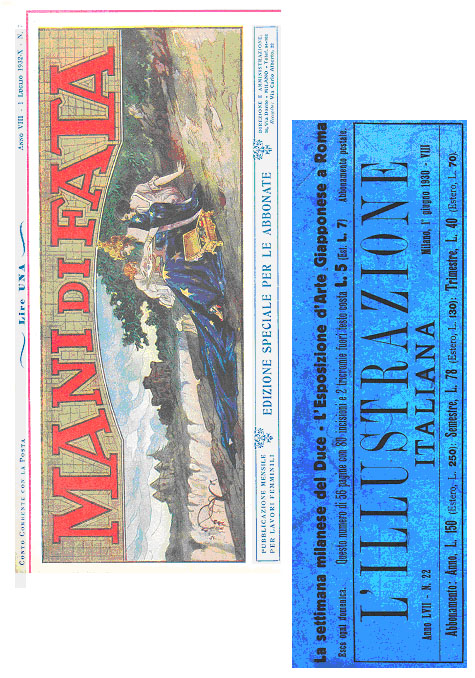
\includegraphics[width=\textwidth]{mani_di_fata.jpg}
	\caption{}
	\label{fig:mani_di_fata}
\end{figure}

\newpage

\begin{figure}[h]
	\centering
		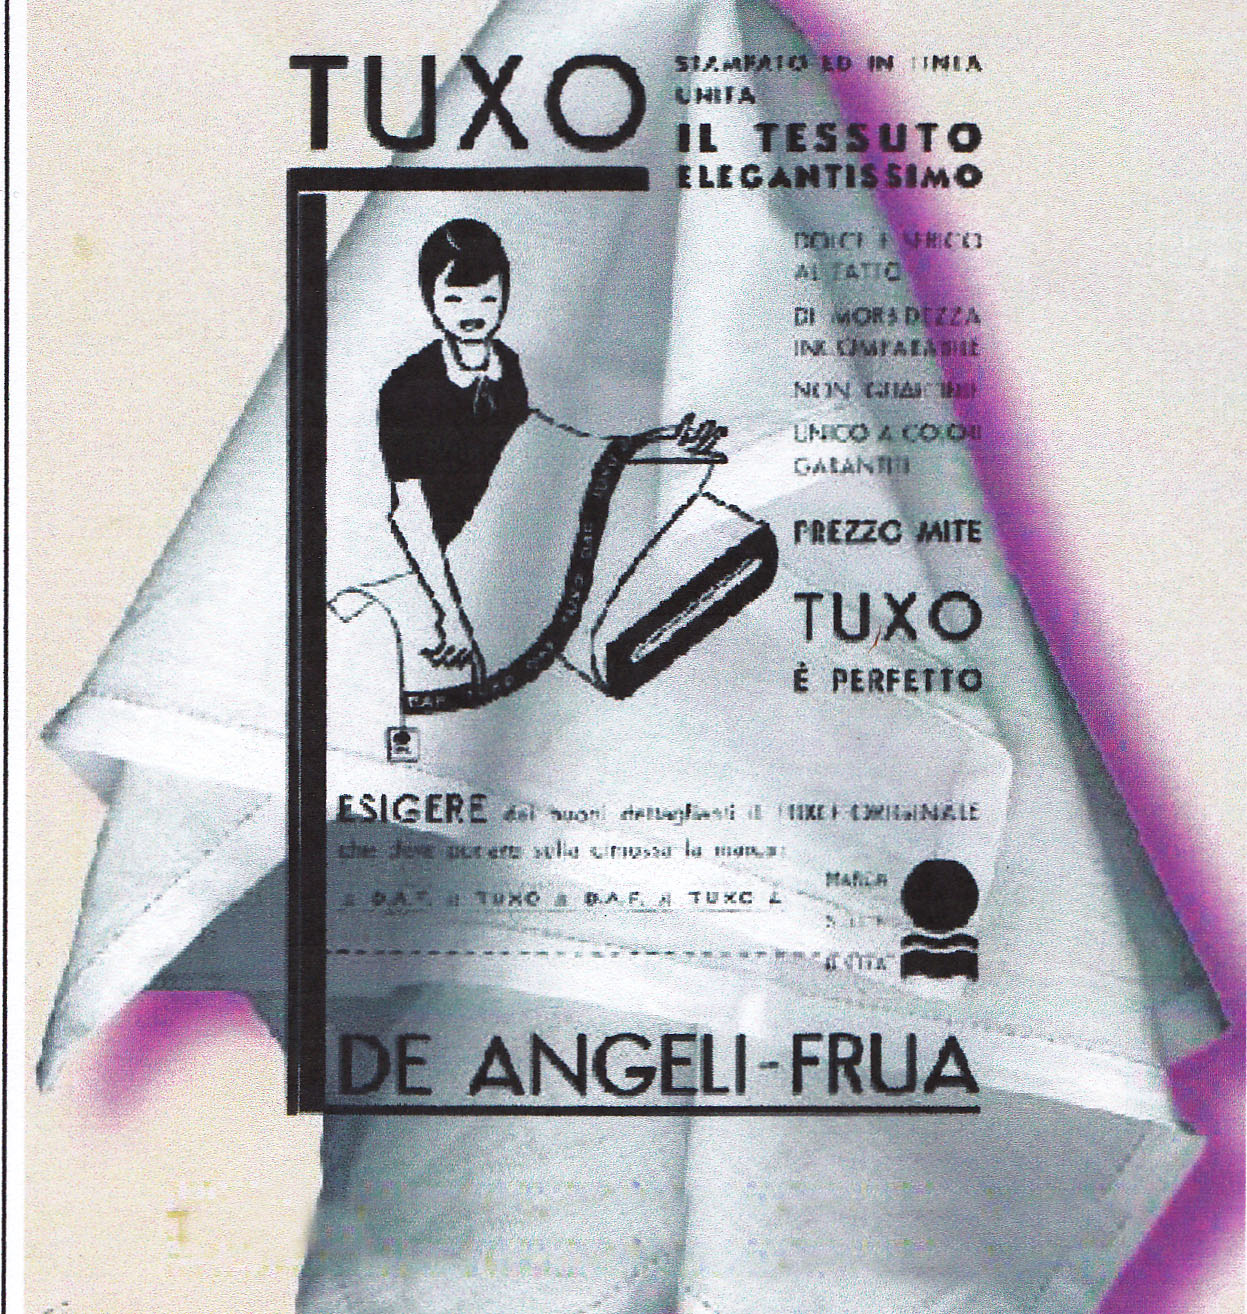
\includegraphics[width=\textwidth]{tuxo.jpg}
	\caption{Da ”Mani di Fata” del dicembre 1932  n° 12}
	\label{fig:tuxo}
\end{figure}

\newpage

\begin{figure}[h]
	\centering
		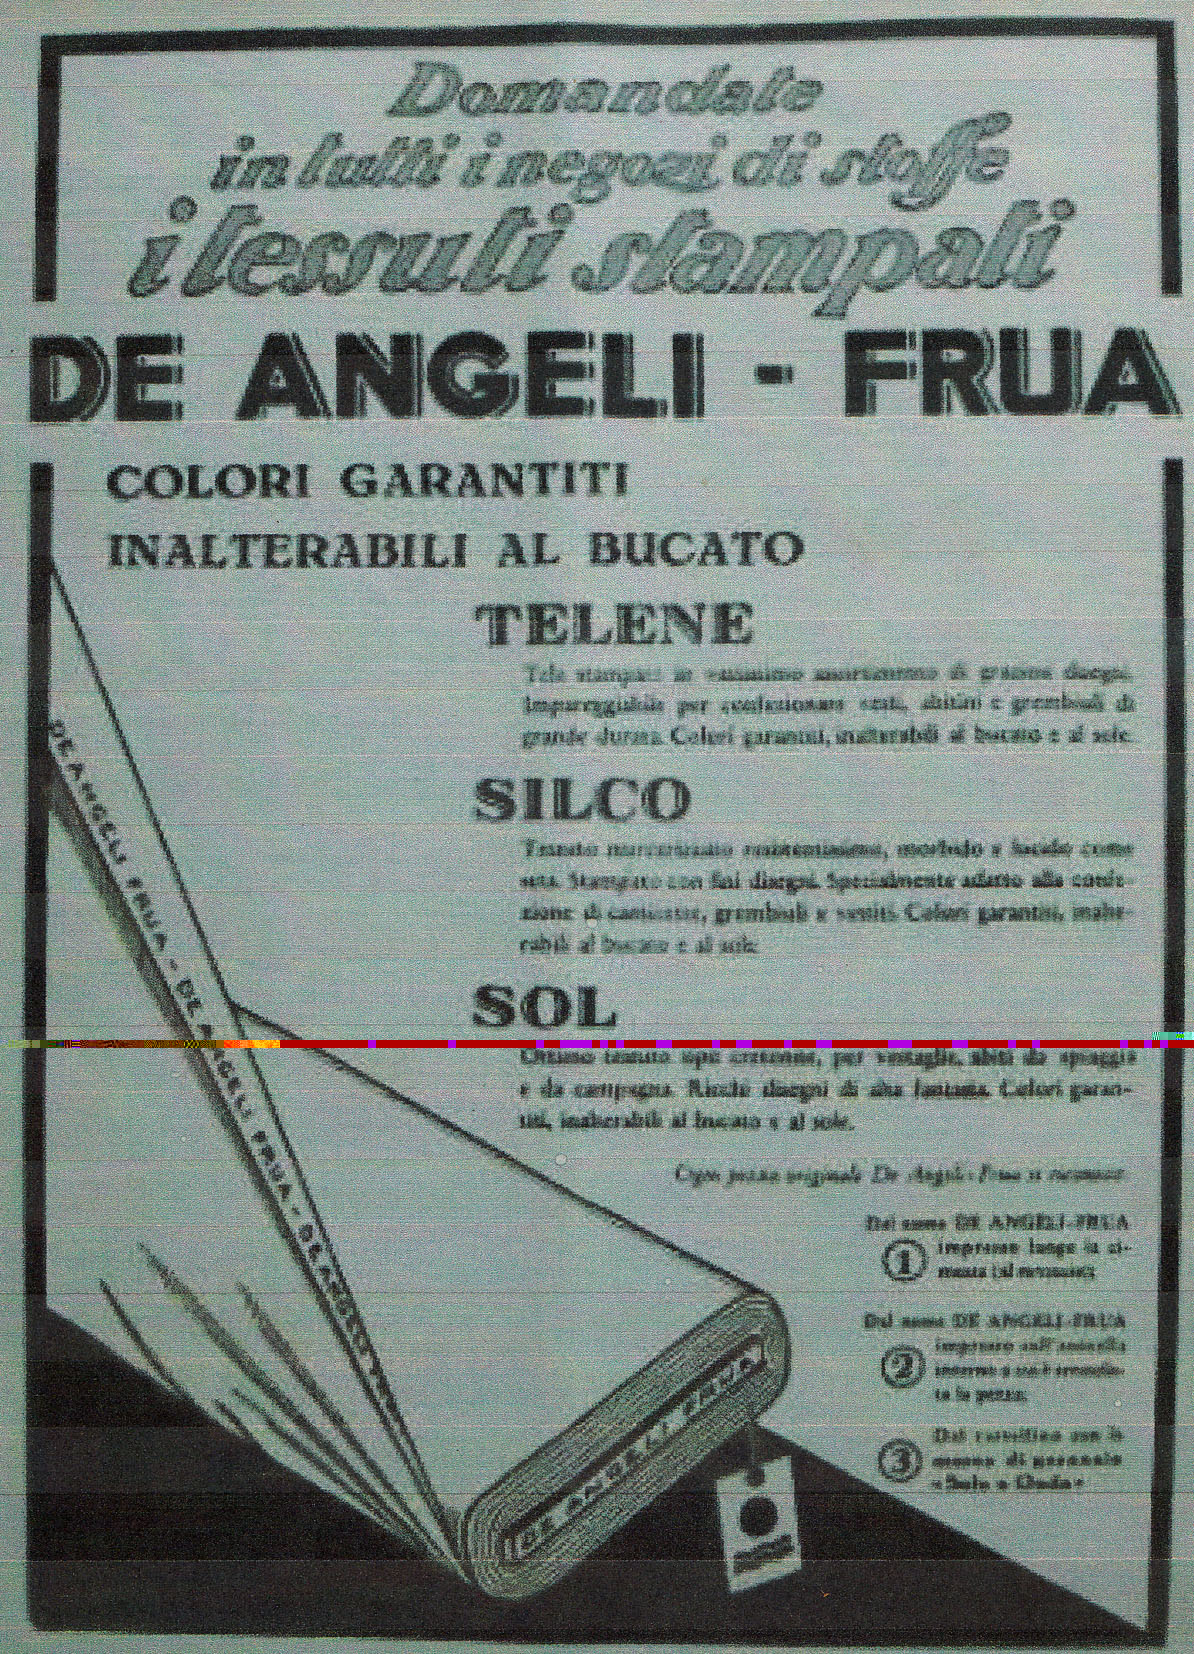
\includegraphics[width=\textwidth]{tessuti_stampati.jpg}
	\caption{Pagina pubblicitaria per tessuti stampati}
	\label{fig:tessuti_stampati}
\end{figure}

\newpage

\begin{figure}[h]
	\centering
		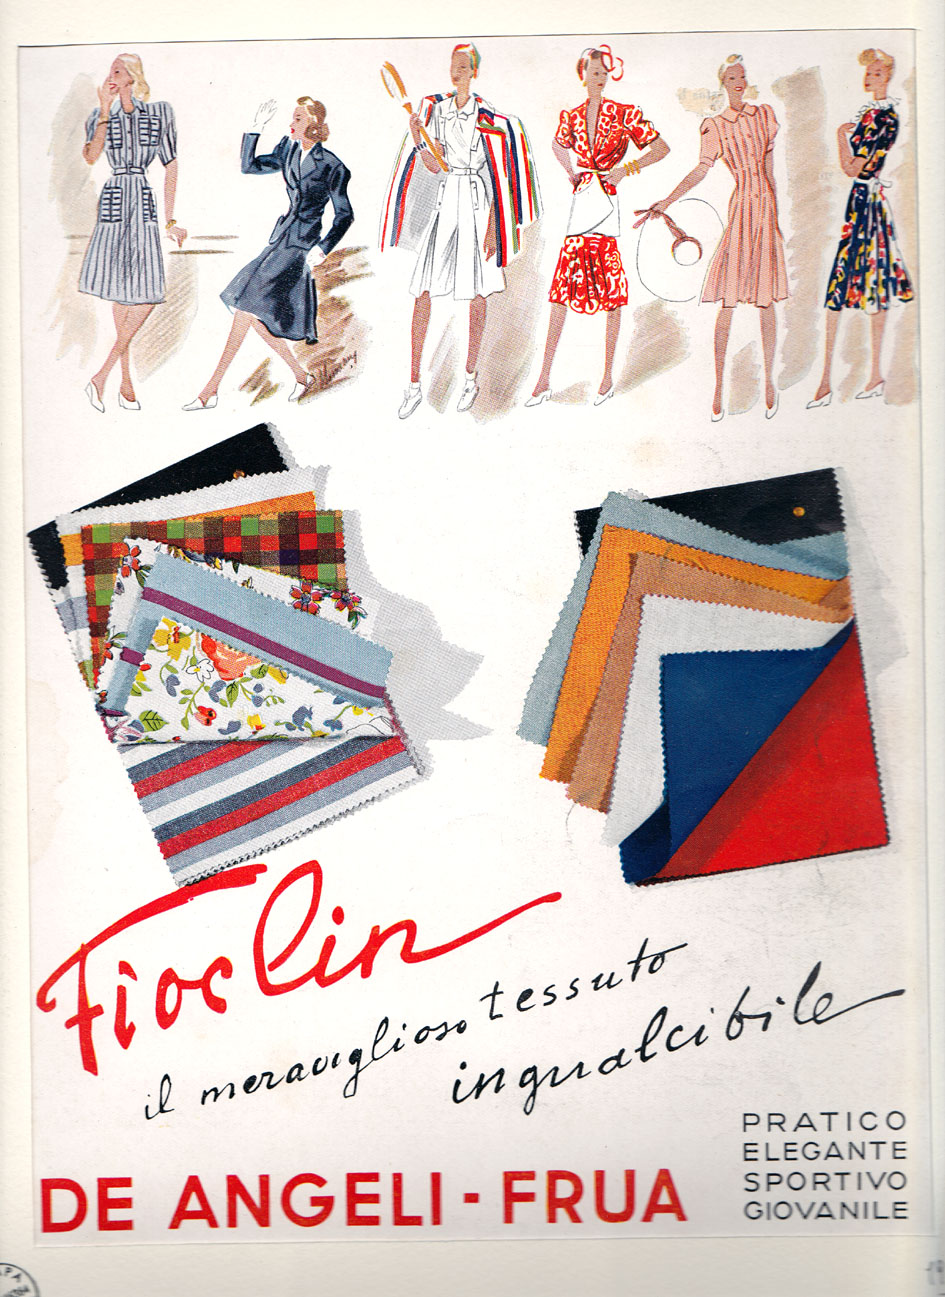
\includegraphics[width=\textwidth]{pagina_pubblicitaria_fioclin.jpg}
	\caption{Pagina pubblicitaria del 1938}
	\label{fig:pagina_pubblicitaria_fioclin}
\end{figure}

\newpage

\begin{figure}[h]
	\centering
		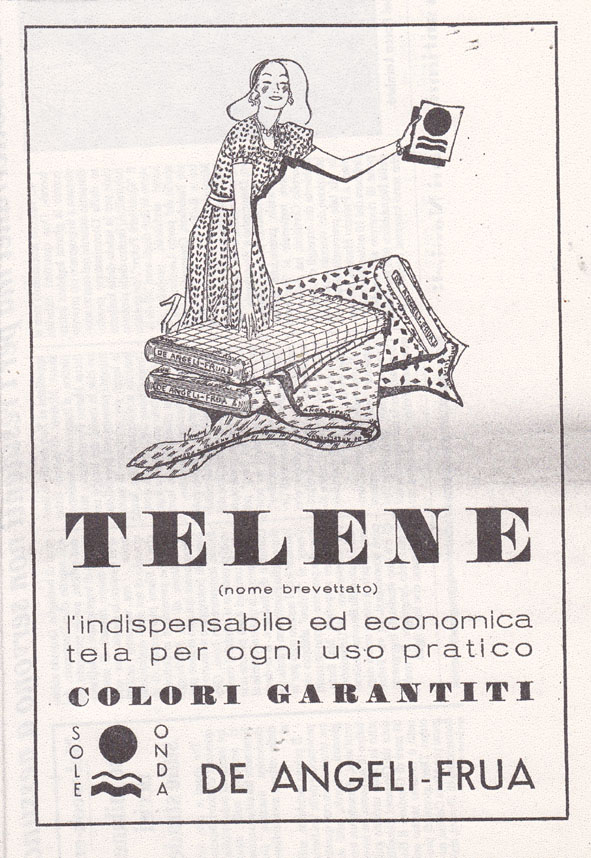
\includegraphics[width=\textwidth]{telene.jpg}
	\caption{Da “Mani di Fata” dell’ agosto 1931, pag. 19}
	\label{fig:telene}
\end{figure}

\newpage

\begin{figure}[h]
	\centering
		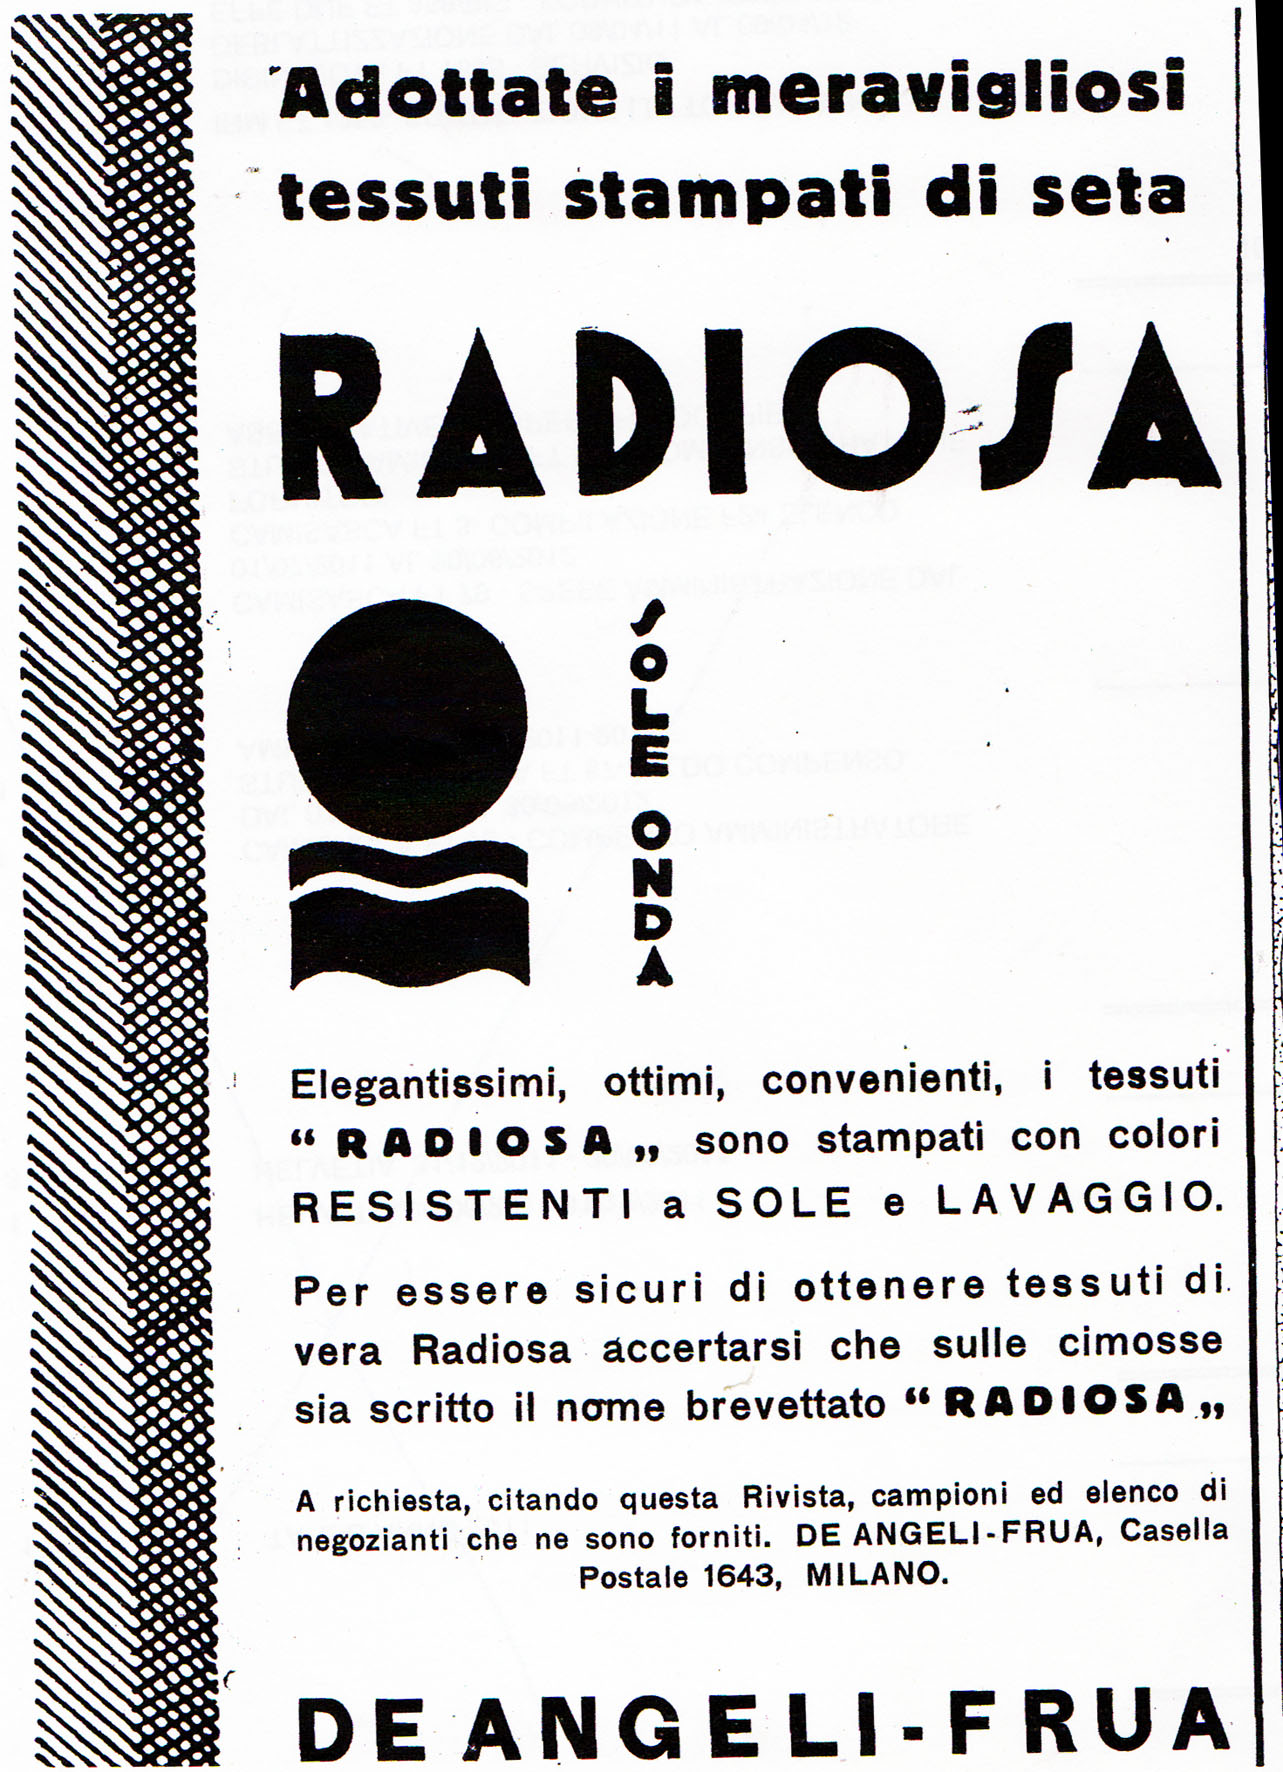
\includegraphics[width=\textwidth]{radiosa.jpg}
	\caption{Da “L’illustrazione italiana” n° 22 del  giugno 1930, pag. 978}
	\label{fig:radiosa}
\end{figure}

\newpage

\begin{figure}[h]
	\centering
		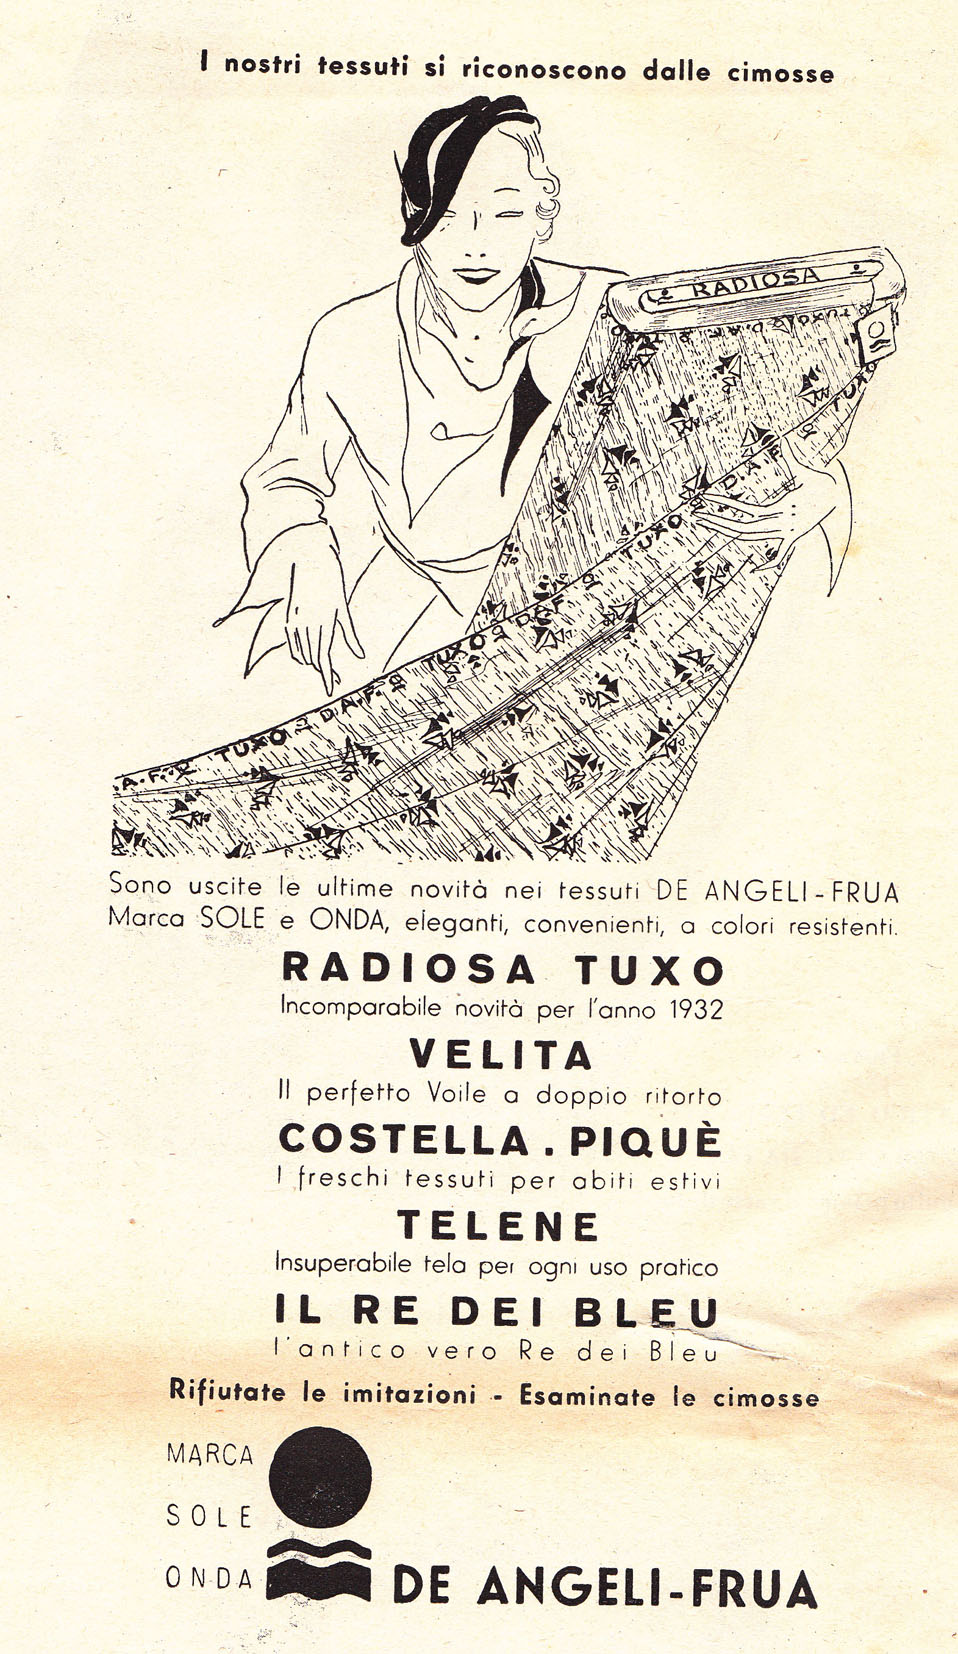
\includegraphics[width=\textwidth]{radiosa_tuxo.jpg}
	\caption{Da “Mani di Fata” del luglio 1932, pag. 15}
	\label{fig:radiosa_tuxo}
\end{figure}

\newpage

\begin{figure}[h]
	\centering
		\includegraphics[width=\textwidth]{vestite_di_tuxo.jpg}
	\caption{Da “Mani di Fata” dell’agosto 1932, pag. 19}
	\label{fig:vestite_di_tuxo}
\end{figure}

\newpage

\begin{figure}[h]
	\centering
		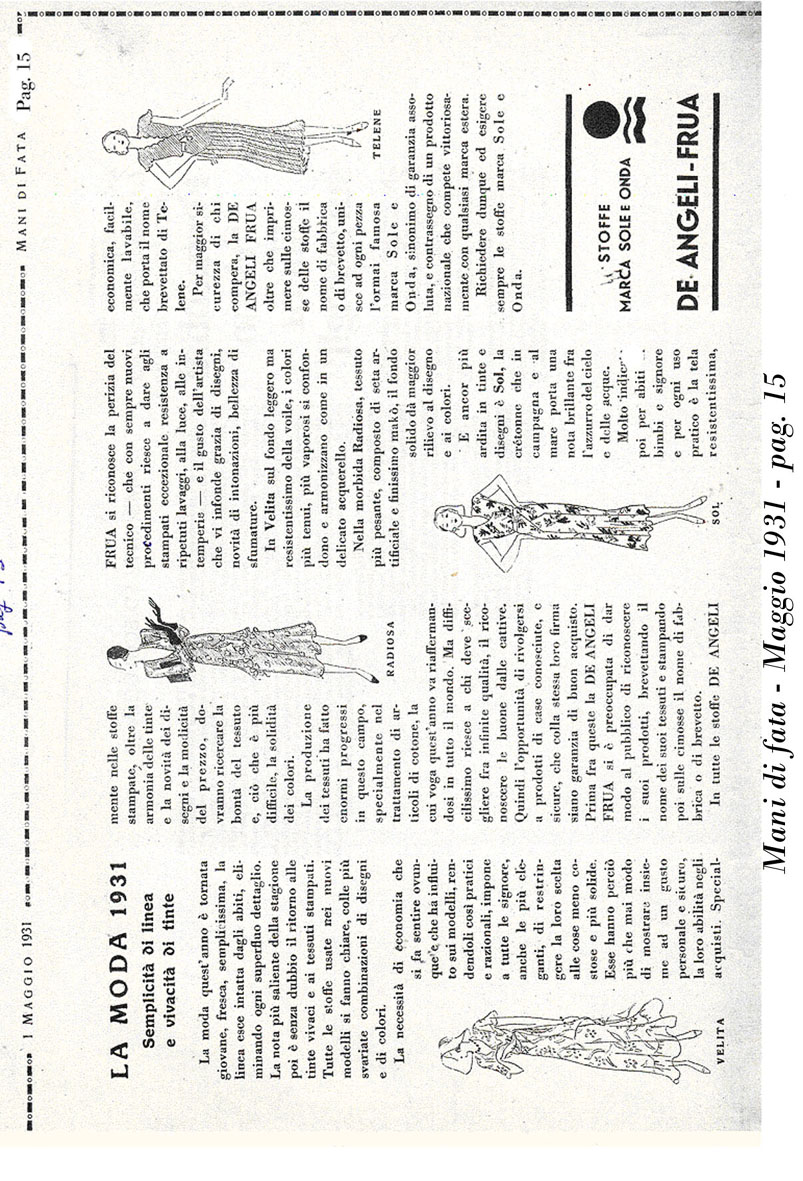
\includegraphics[width=\textwidth]{la_moda.jpg}
	\caption{}
	\label{fig:la_moda}
\end{figure}

\newpage

\begin{figure}[h]
	\centering
		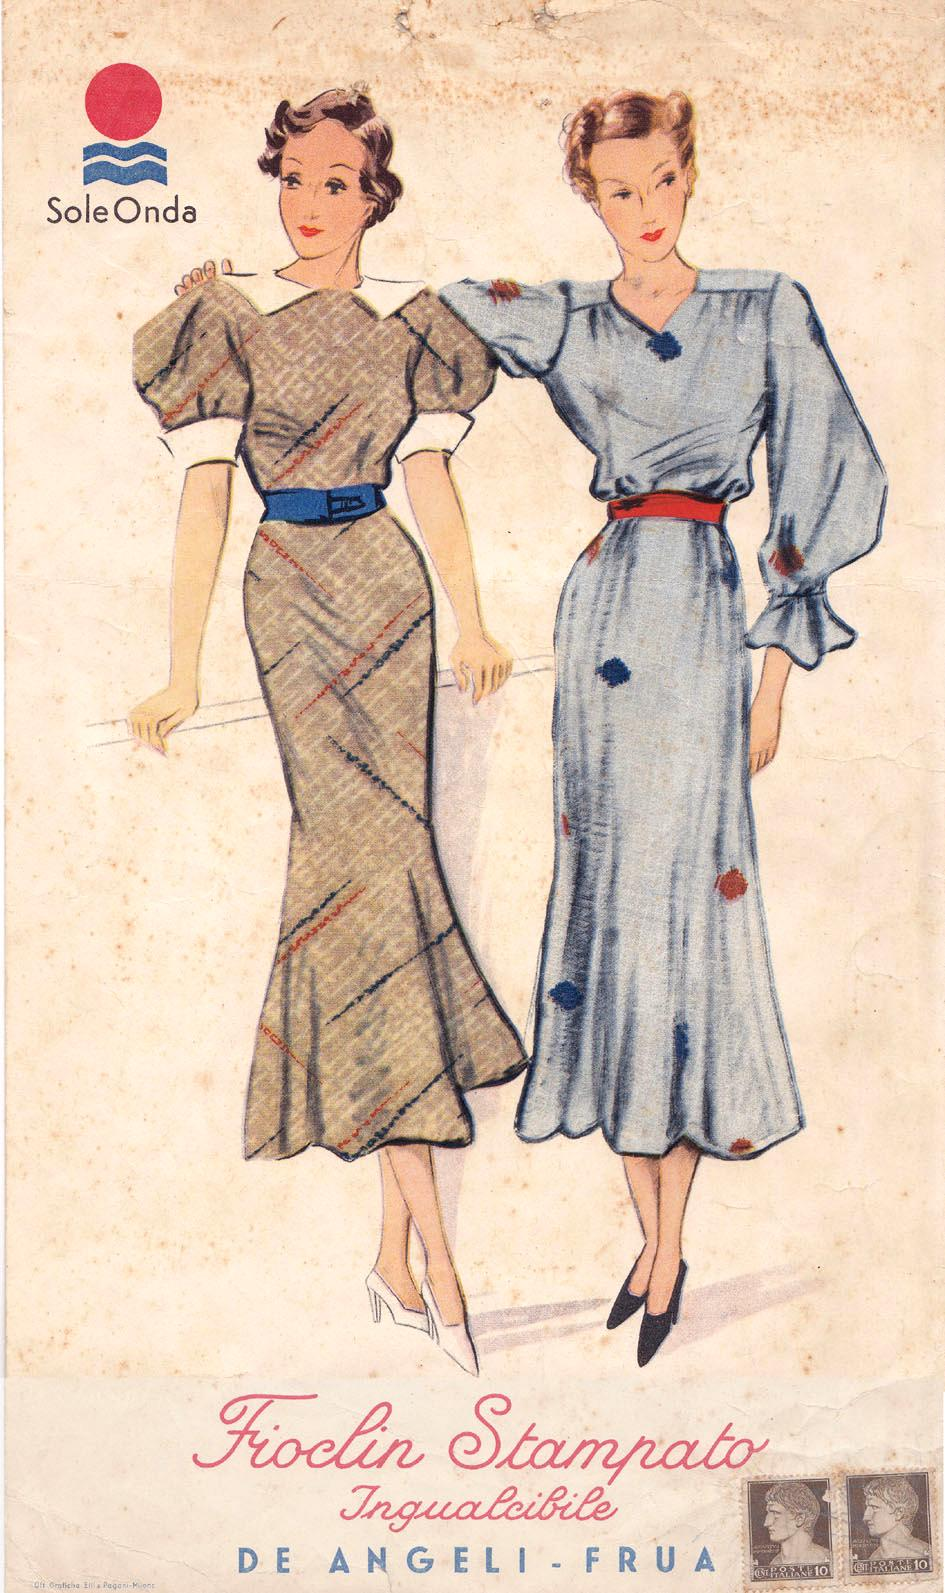
\includegraphics[width=\textwidth]{locandina.jpg}
	\caption{Locandina tranviaria}
	\label{fig:locandina}
\end{figure}

\newpage

\begin{figure}[h]
	\centering
		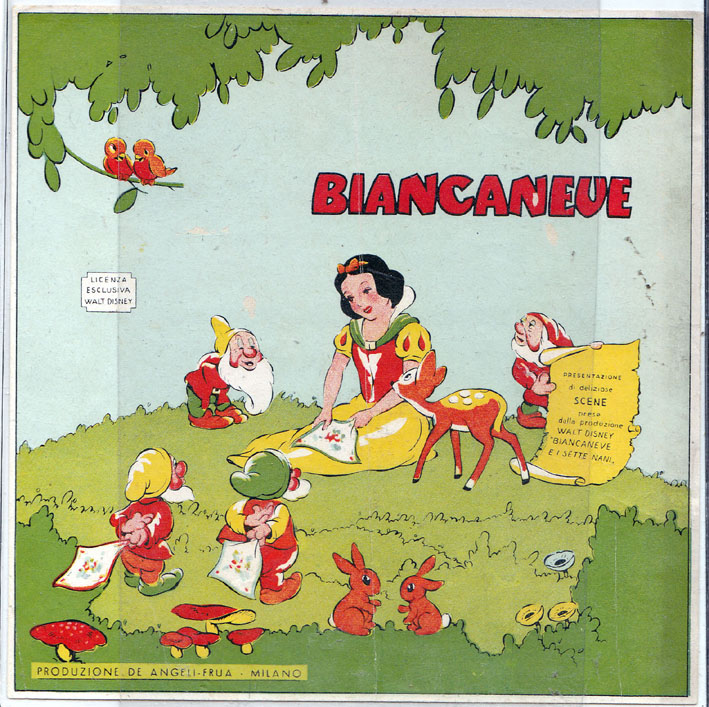
\includegraphics[width=\textwidth]{biancaneve.jpg}
	\caption{Produzione di fazzoletti con personaggi Walt Disney}
	\label{fig:biancaneve}
\end{figure}
\begin{figure}[h]
	\centering
		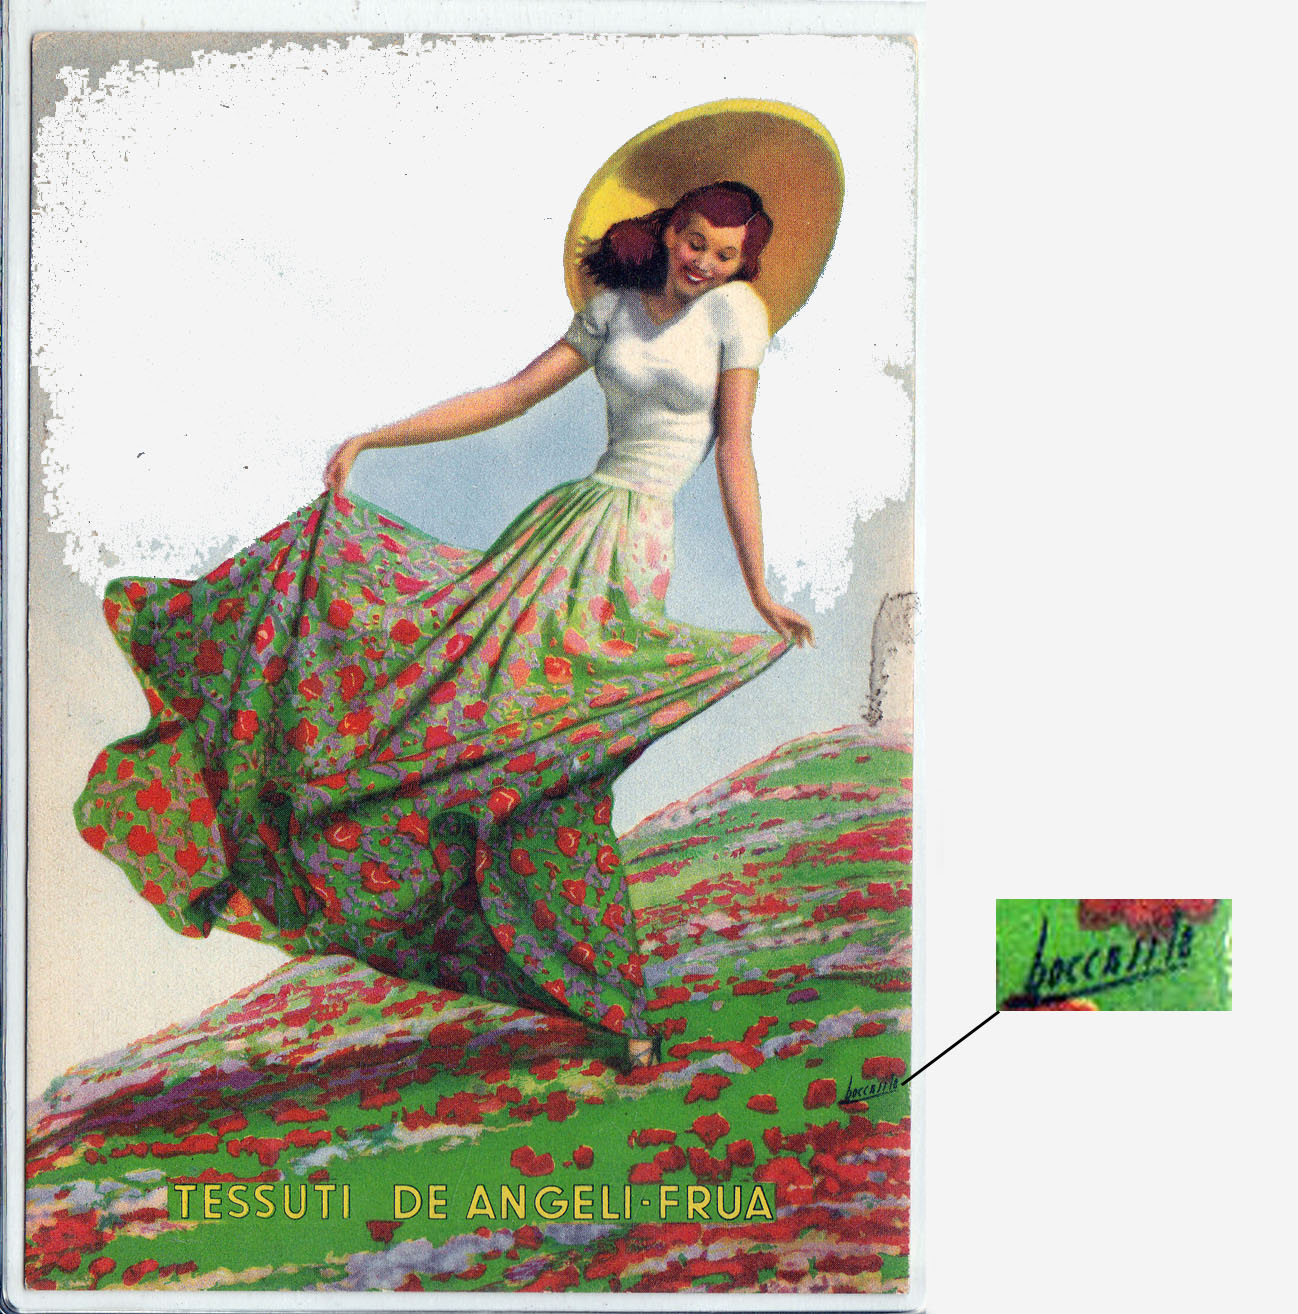
\includegraphics[width=\textwidth]{boccasile.jpg}
	\caption{Cartolina a firma Boccasile}
	\label{fig:boccasile}
\end{figure}

\newpage

Serie di sei cartoline pubblicitarie emesse nel 1939

\begin{figure}[h]
	\centering
		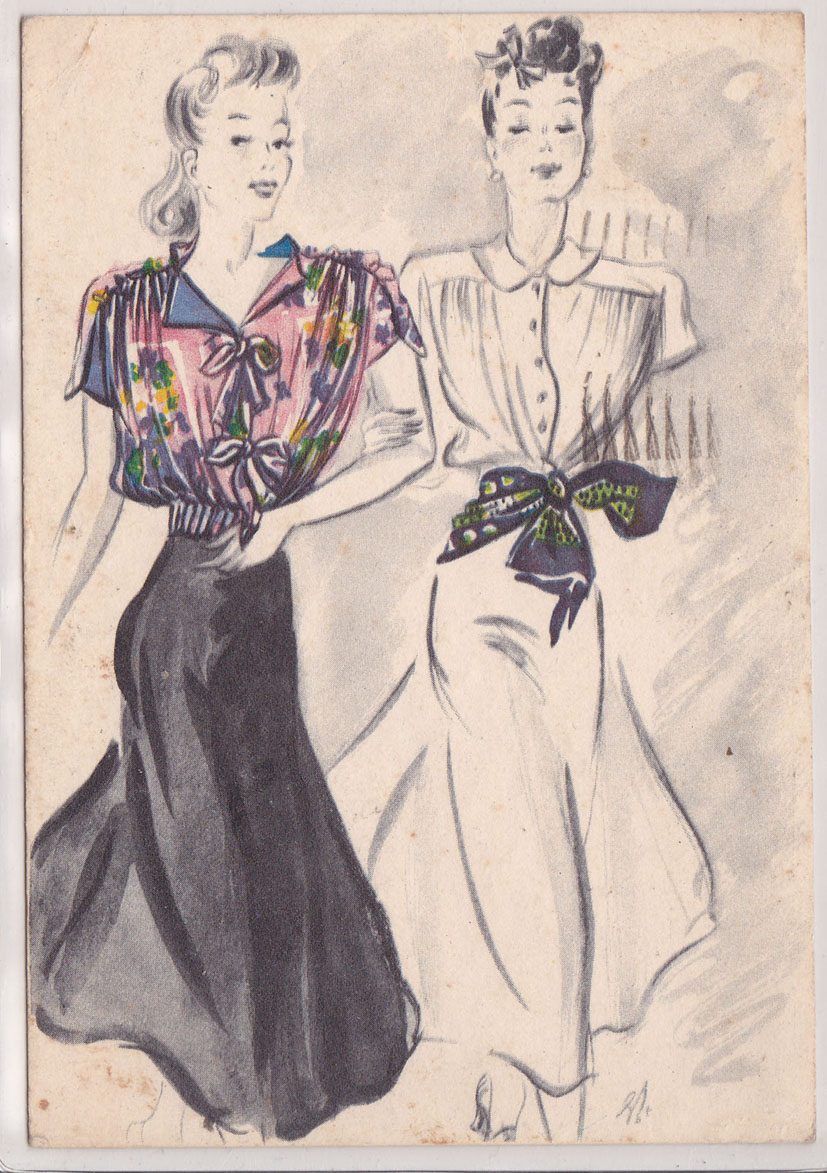
\includegraphics[width=\textwidth]{cartolina_1.jpg}
	\caption{}
	\label{fig:cartolina_1}
\end{figure}
\begin{figure}[h]
	\centering
		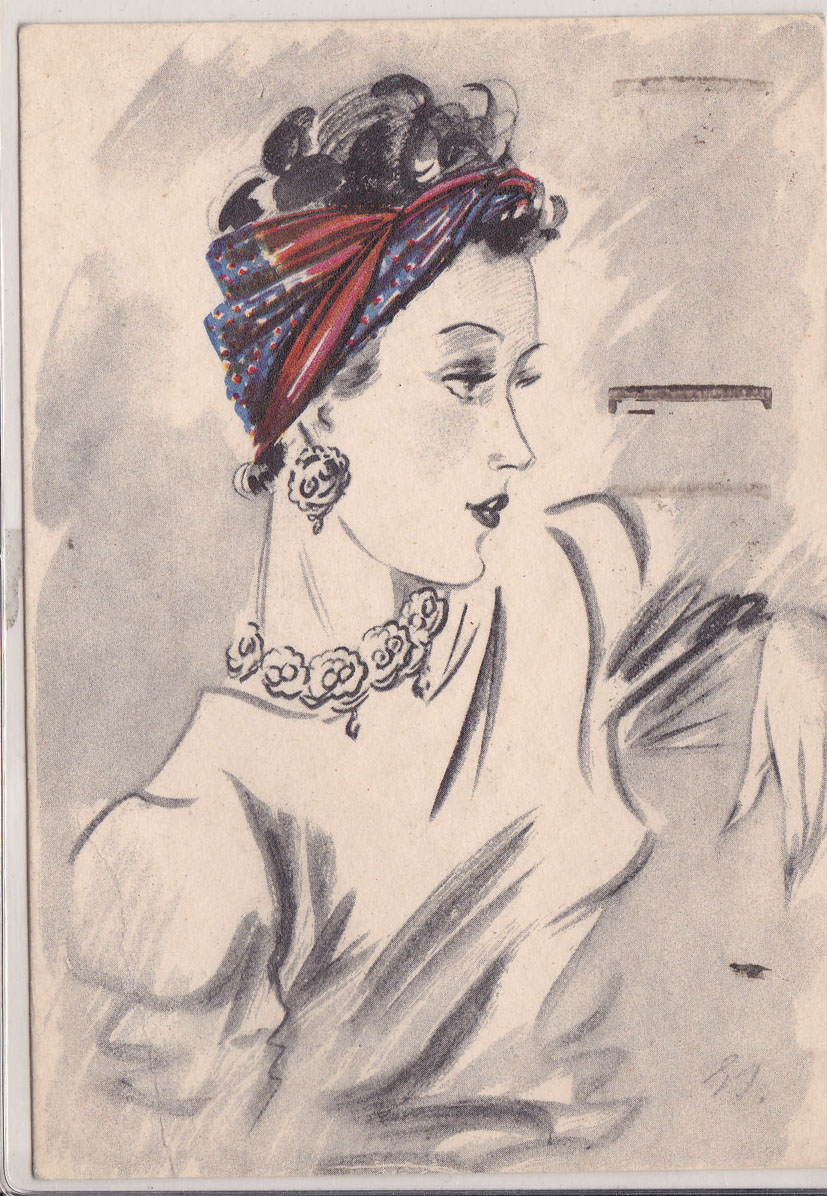
\includegraphics[width=\textwidth]{cartolina_2.jpg}
	\caption{}
	\label{fig:cartolina_2}
\end{figure}

\newpage

\begin{figure}[h]
	\centering
		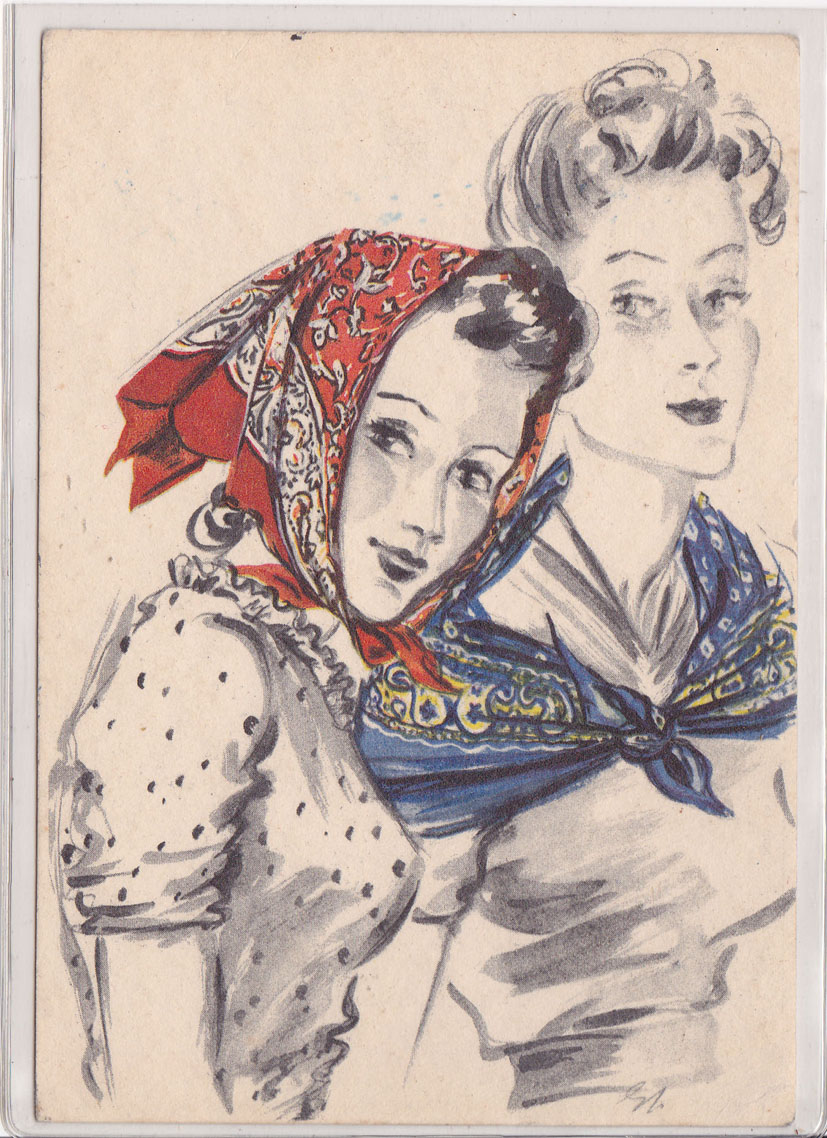
\includegraphics[width=\textwidth]{cartolina_3.jpg}
	\caption{}
	\label{fig:cartolina_3}
\end{figure}
\begin{figure}[h]
	\centering
		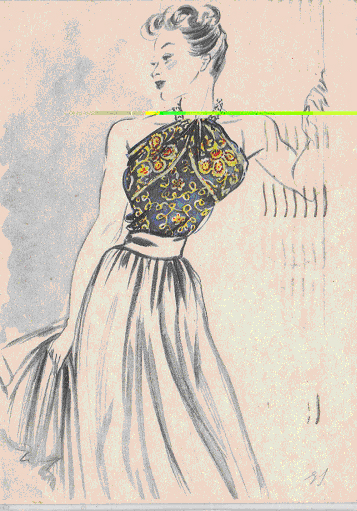
\includegraphics[width=\textwidth]{cartolina_4.jpg}
	\caption{}
	\label{fig:cartolina_4}
\end{figure}

\newpage

\begin{figure}[h]
	\centering
		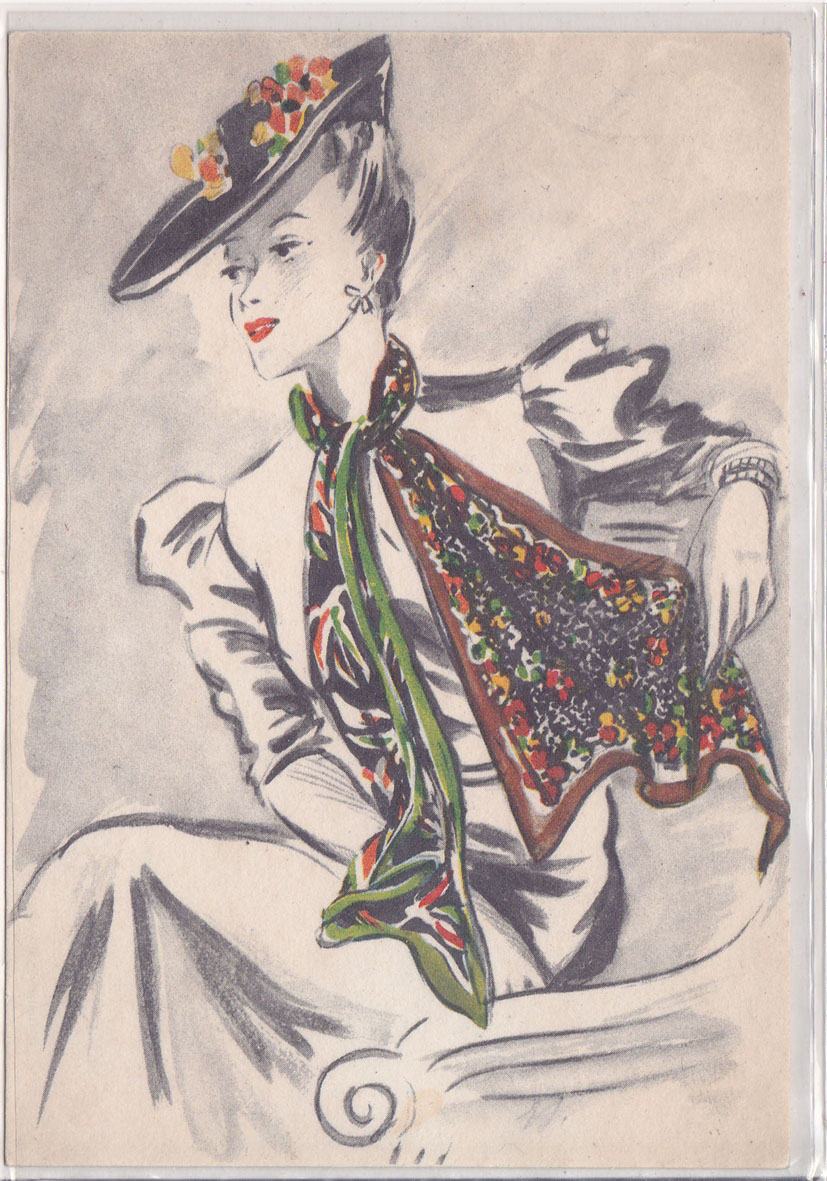
\includegraphics[width=\textwidth]{cartolina_5.jpg}
	\caption{}
	\label{fig:cartolina_5}
\end{figure}
\begin{figure}[h]
	\centering
		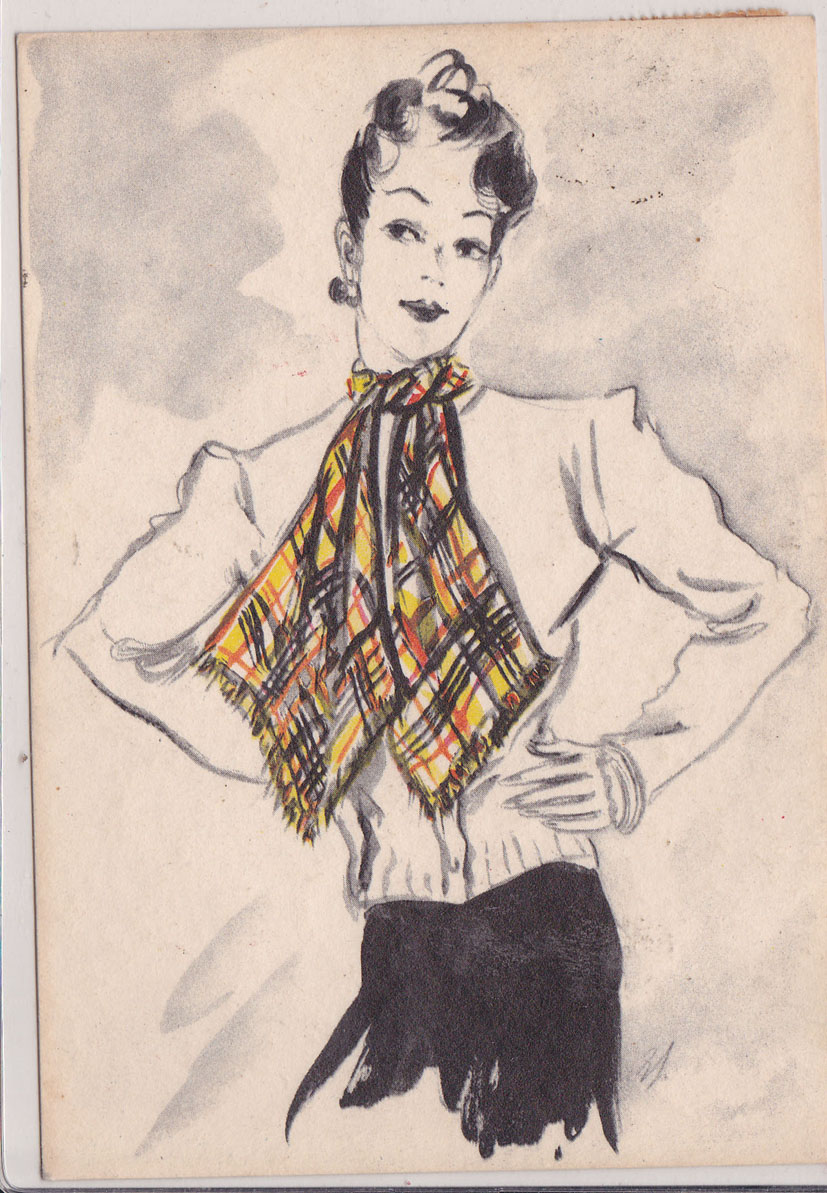
\includegraphics[width=\textwidth]{cartolina_6.jpg}
	\caption{}
	\label{fig:cartolina_6}
\end{figure}

\newpage

\begin{figure}[h]
	\centering
		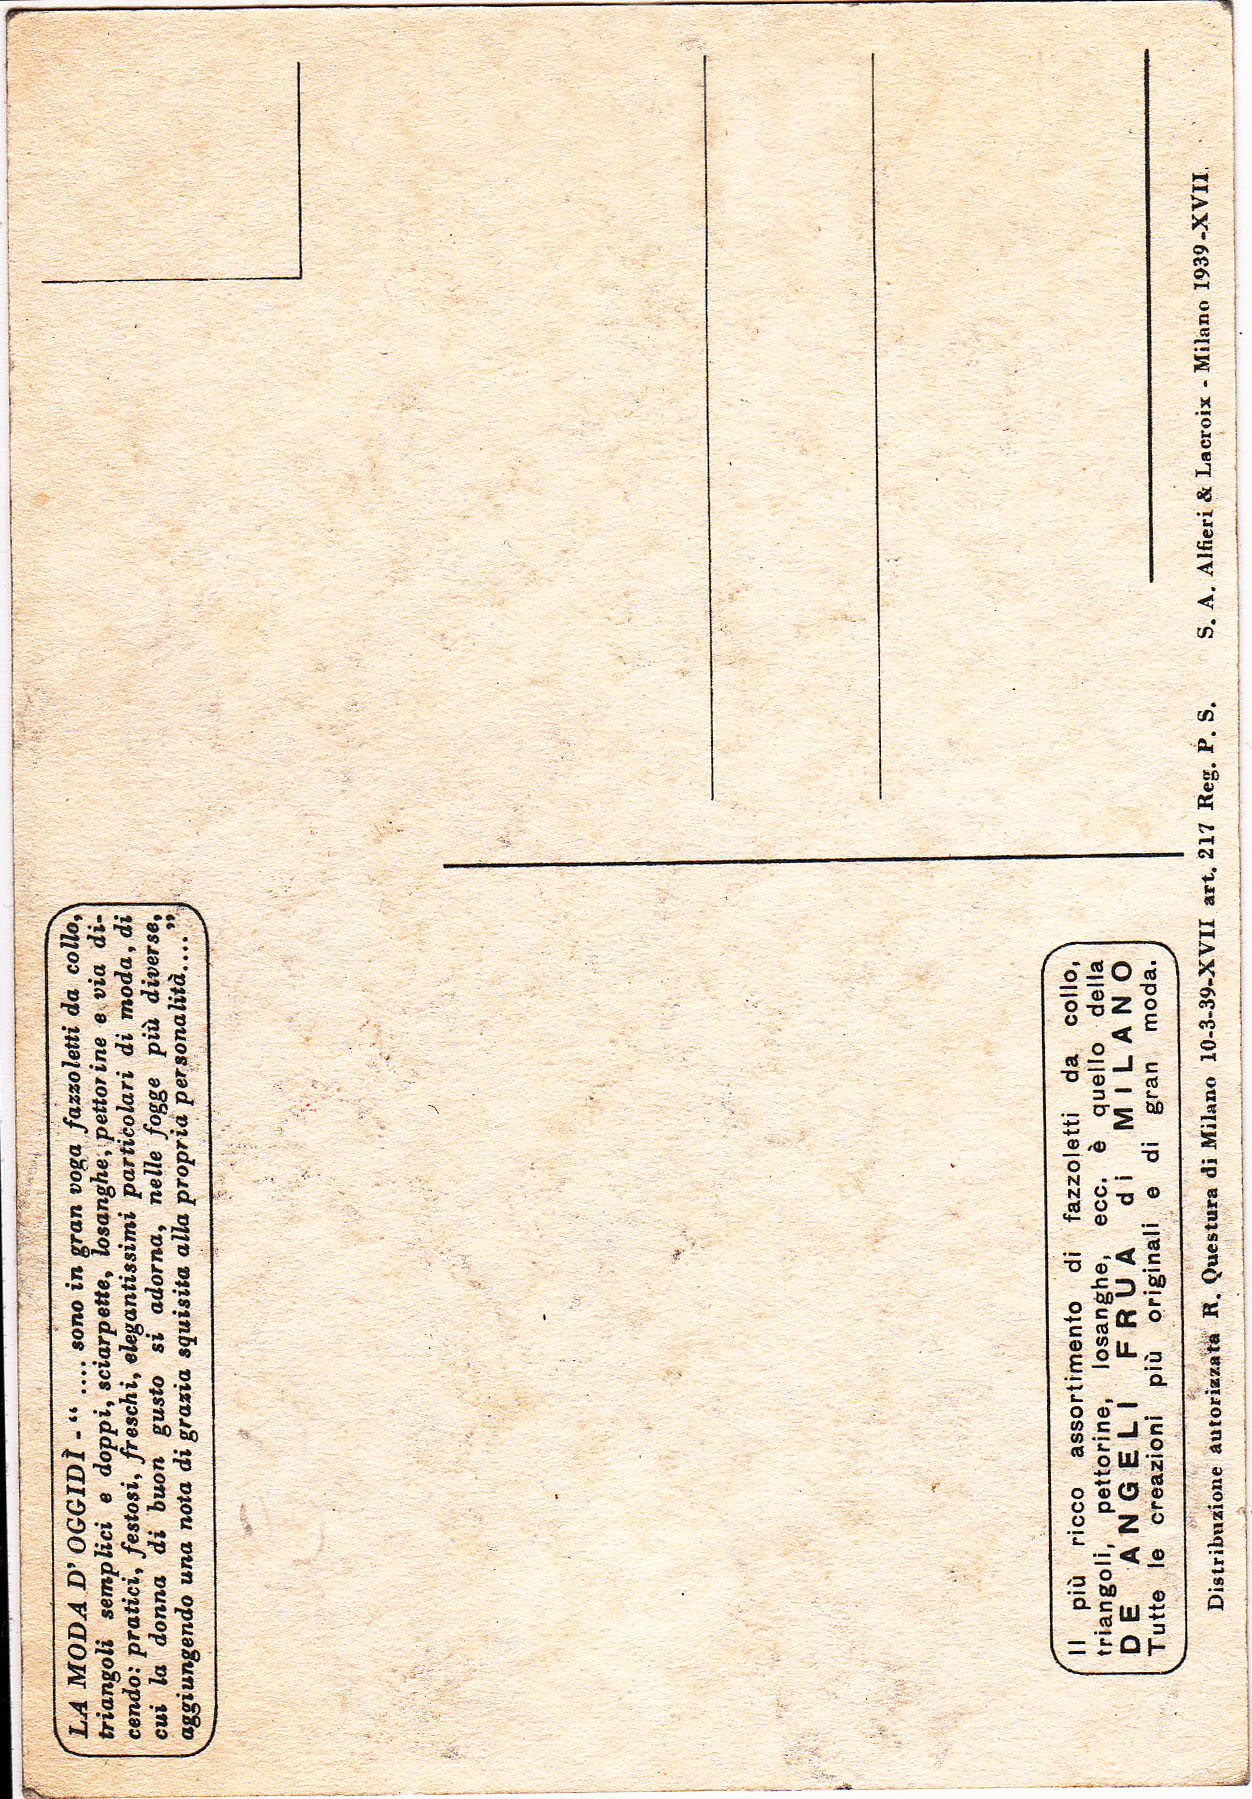
\includegraphics[width=\textwidth]{cartolina_finale.jpg}
	\caption{Stampigliatura sul retro delle sei  cartoline pubblicitarie}
	\label{fig:cartolina_finale}
\end{figure}

\newpage

\begin{figure}[h]
	\centering
		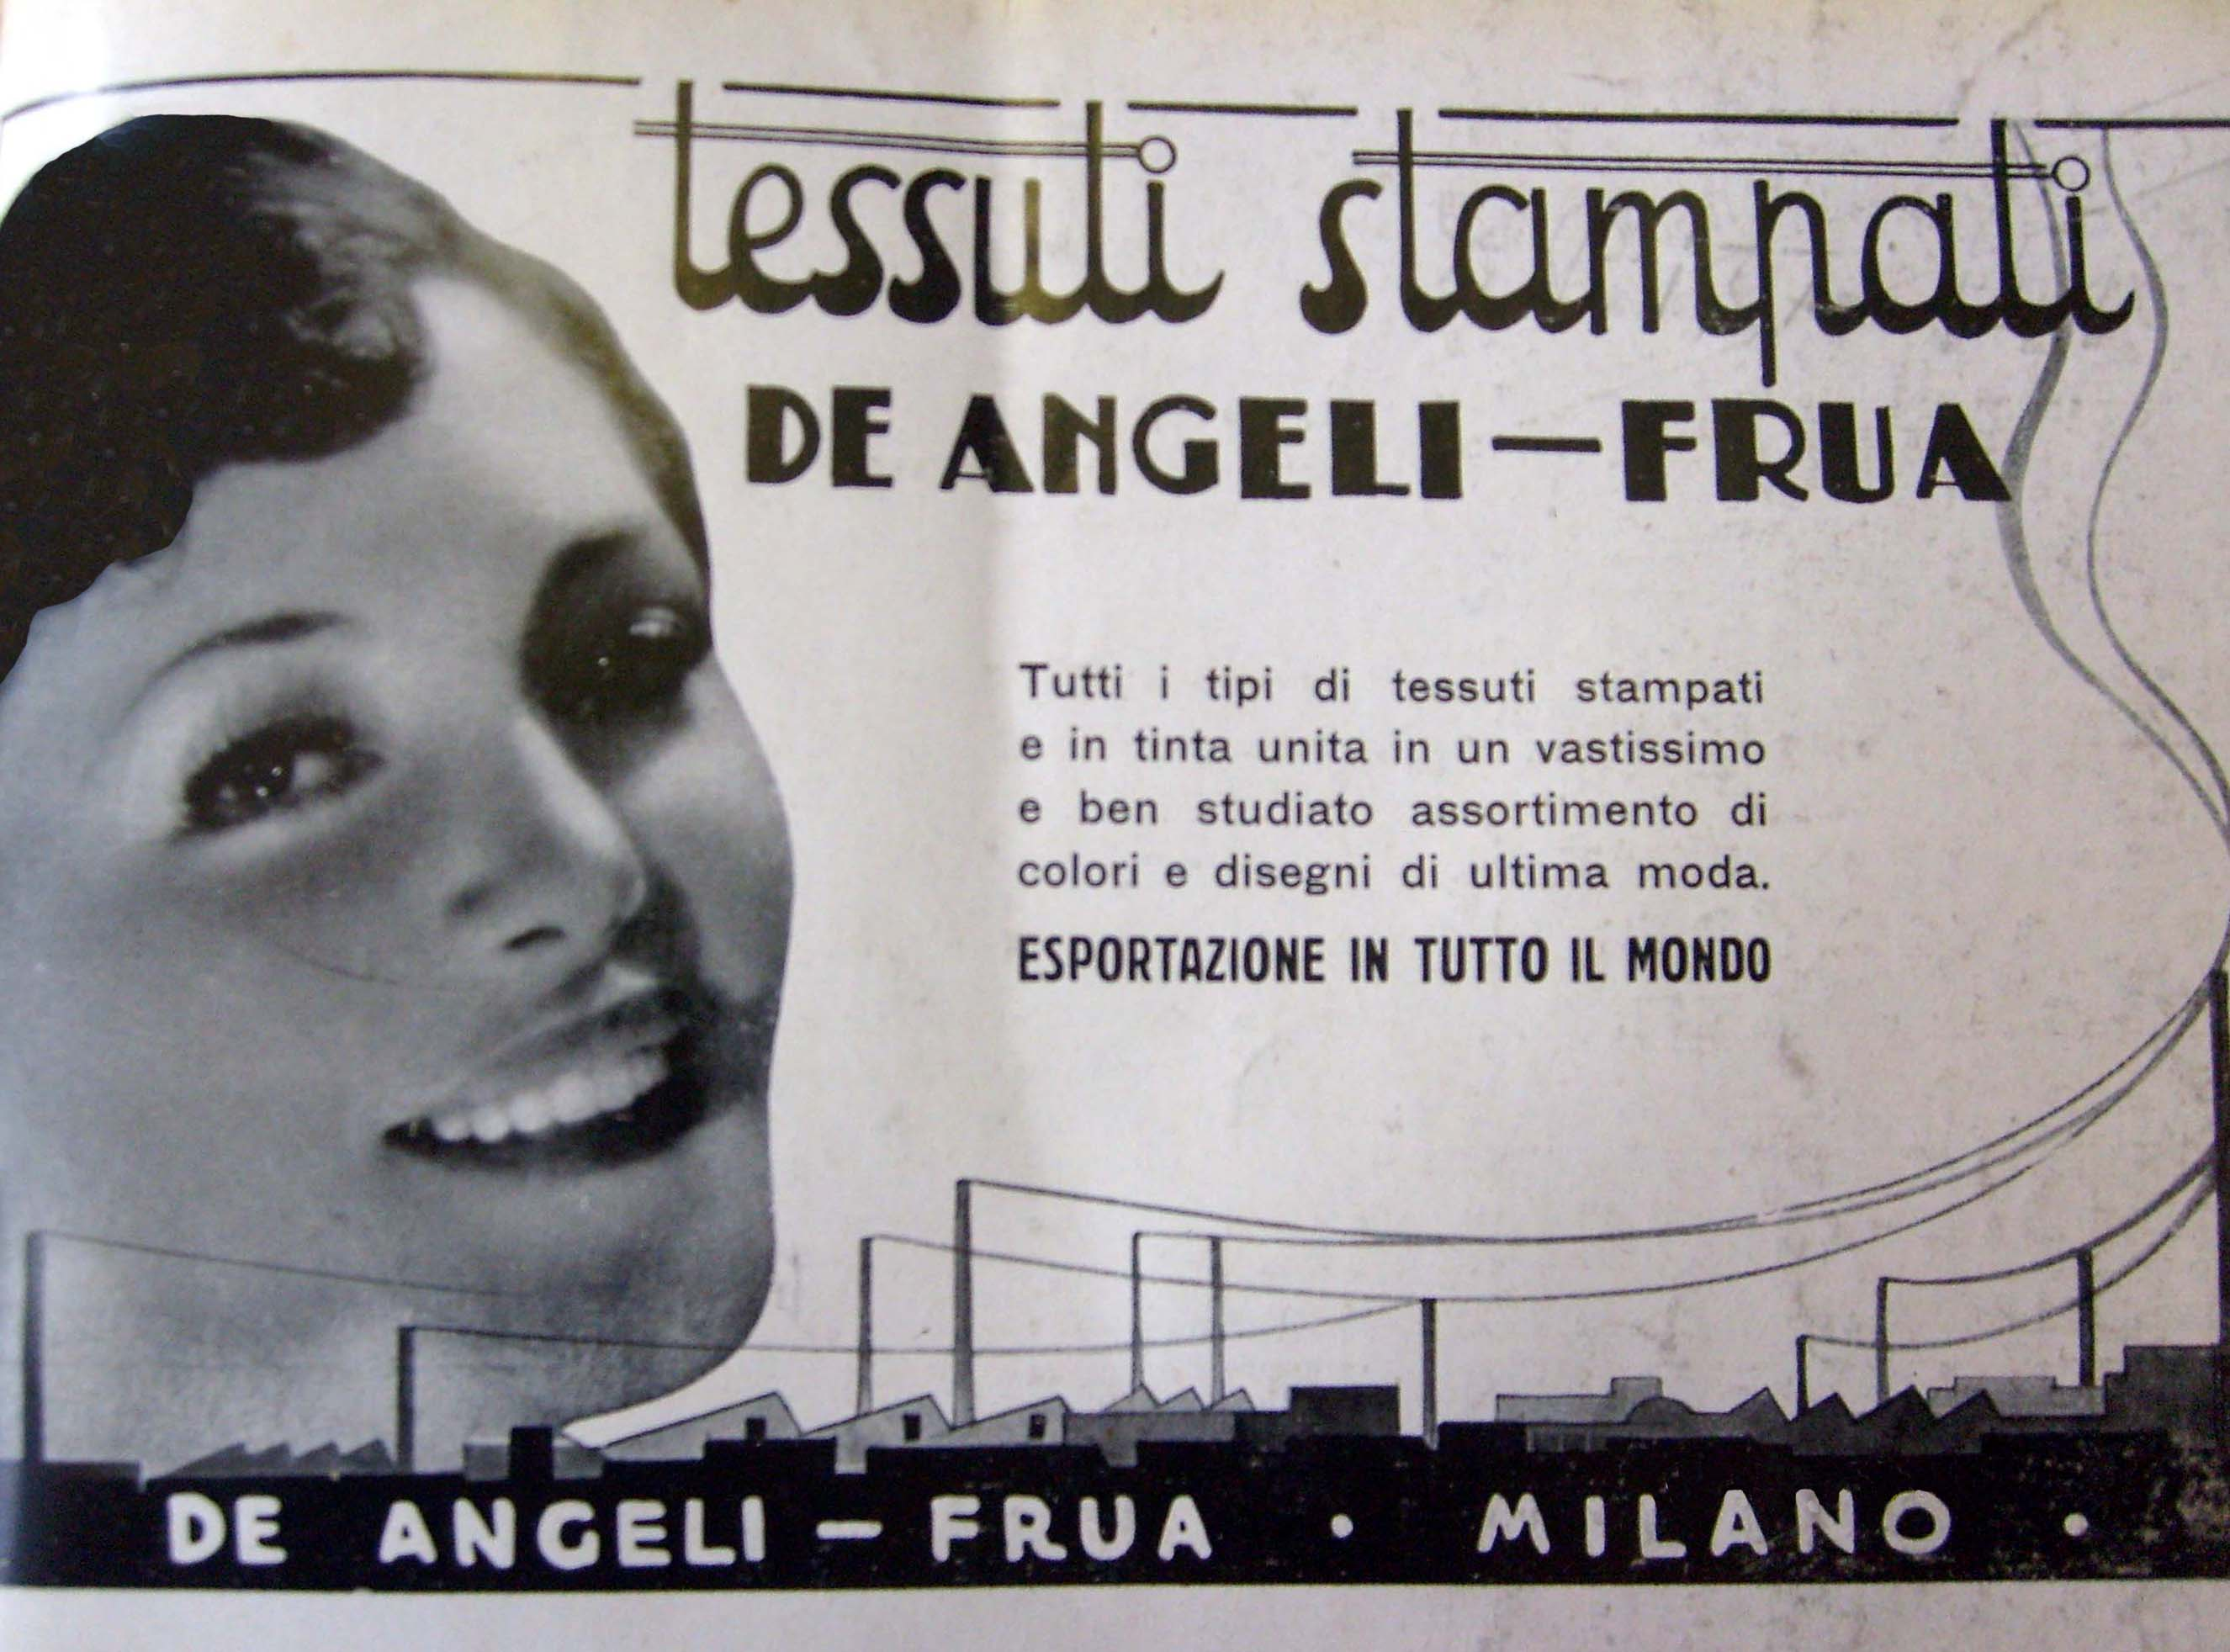
\includegraphics[width=\textwidth]{deangeli_1.jpg}
	\caption{}
	\label{fig:deangeli_1}
\end{figure}
\begin{figure}[h]
	\centering
		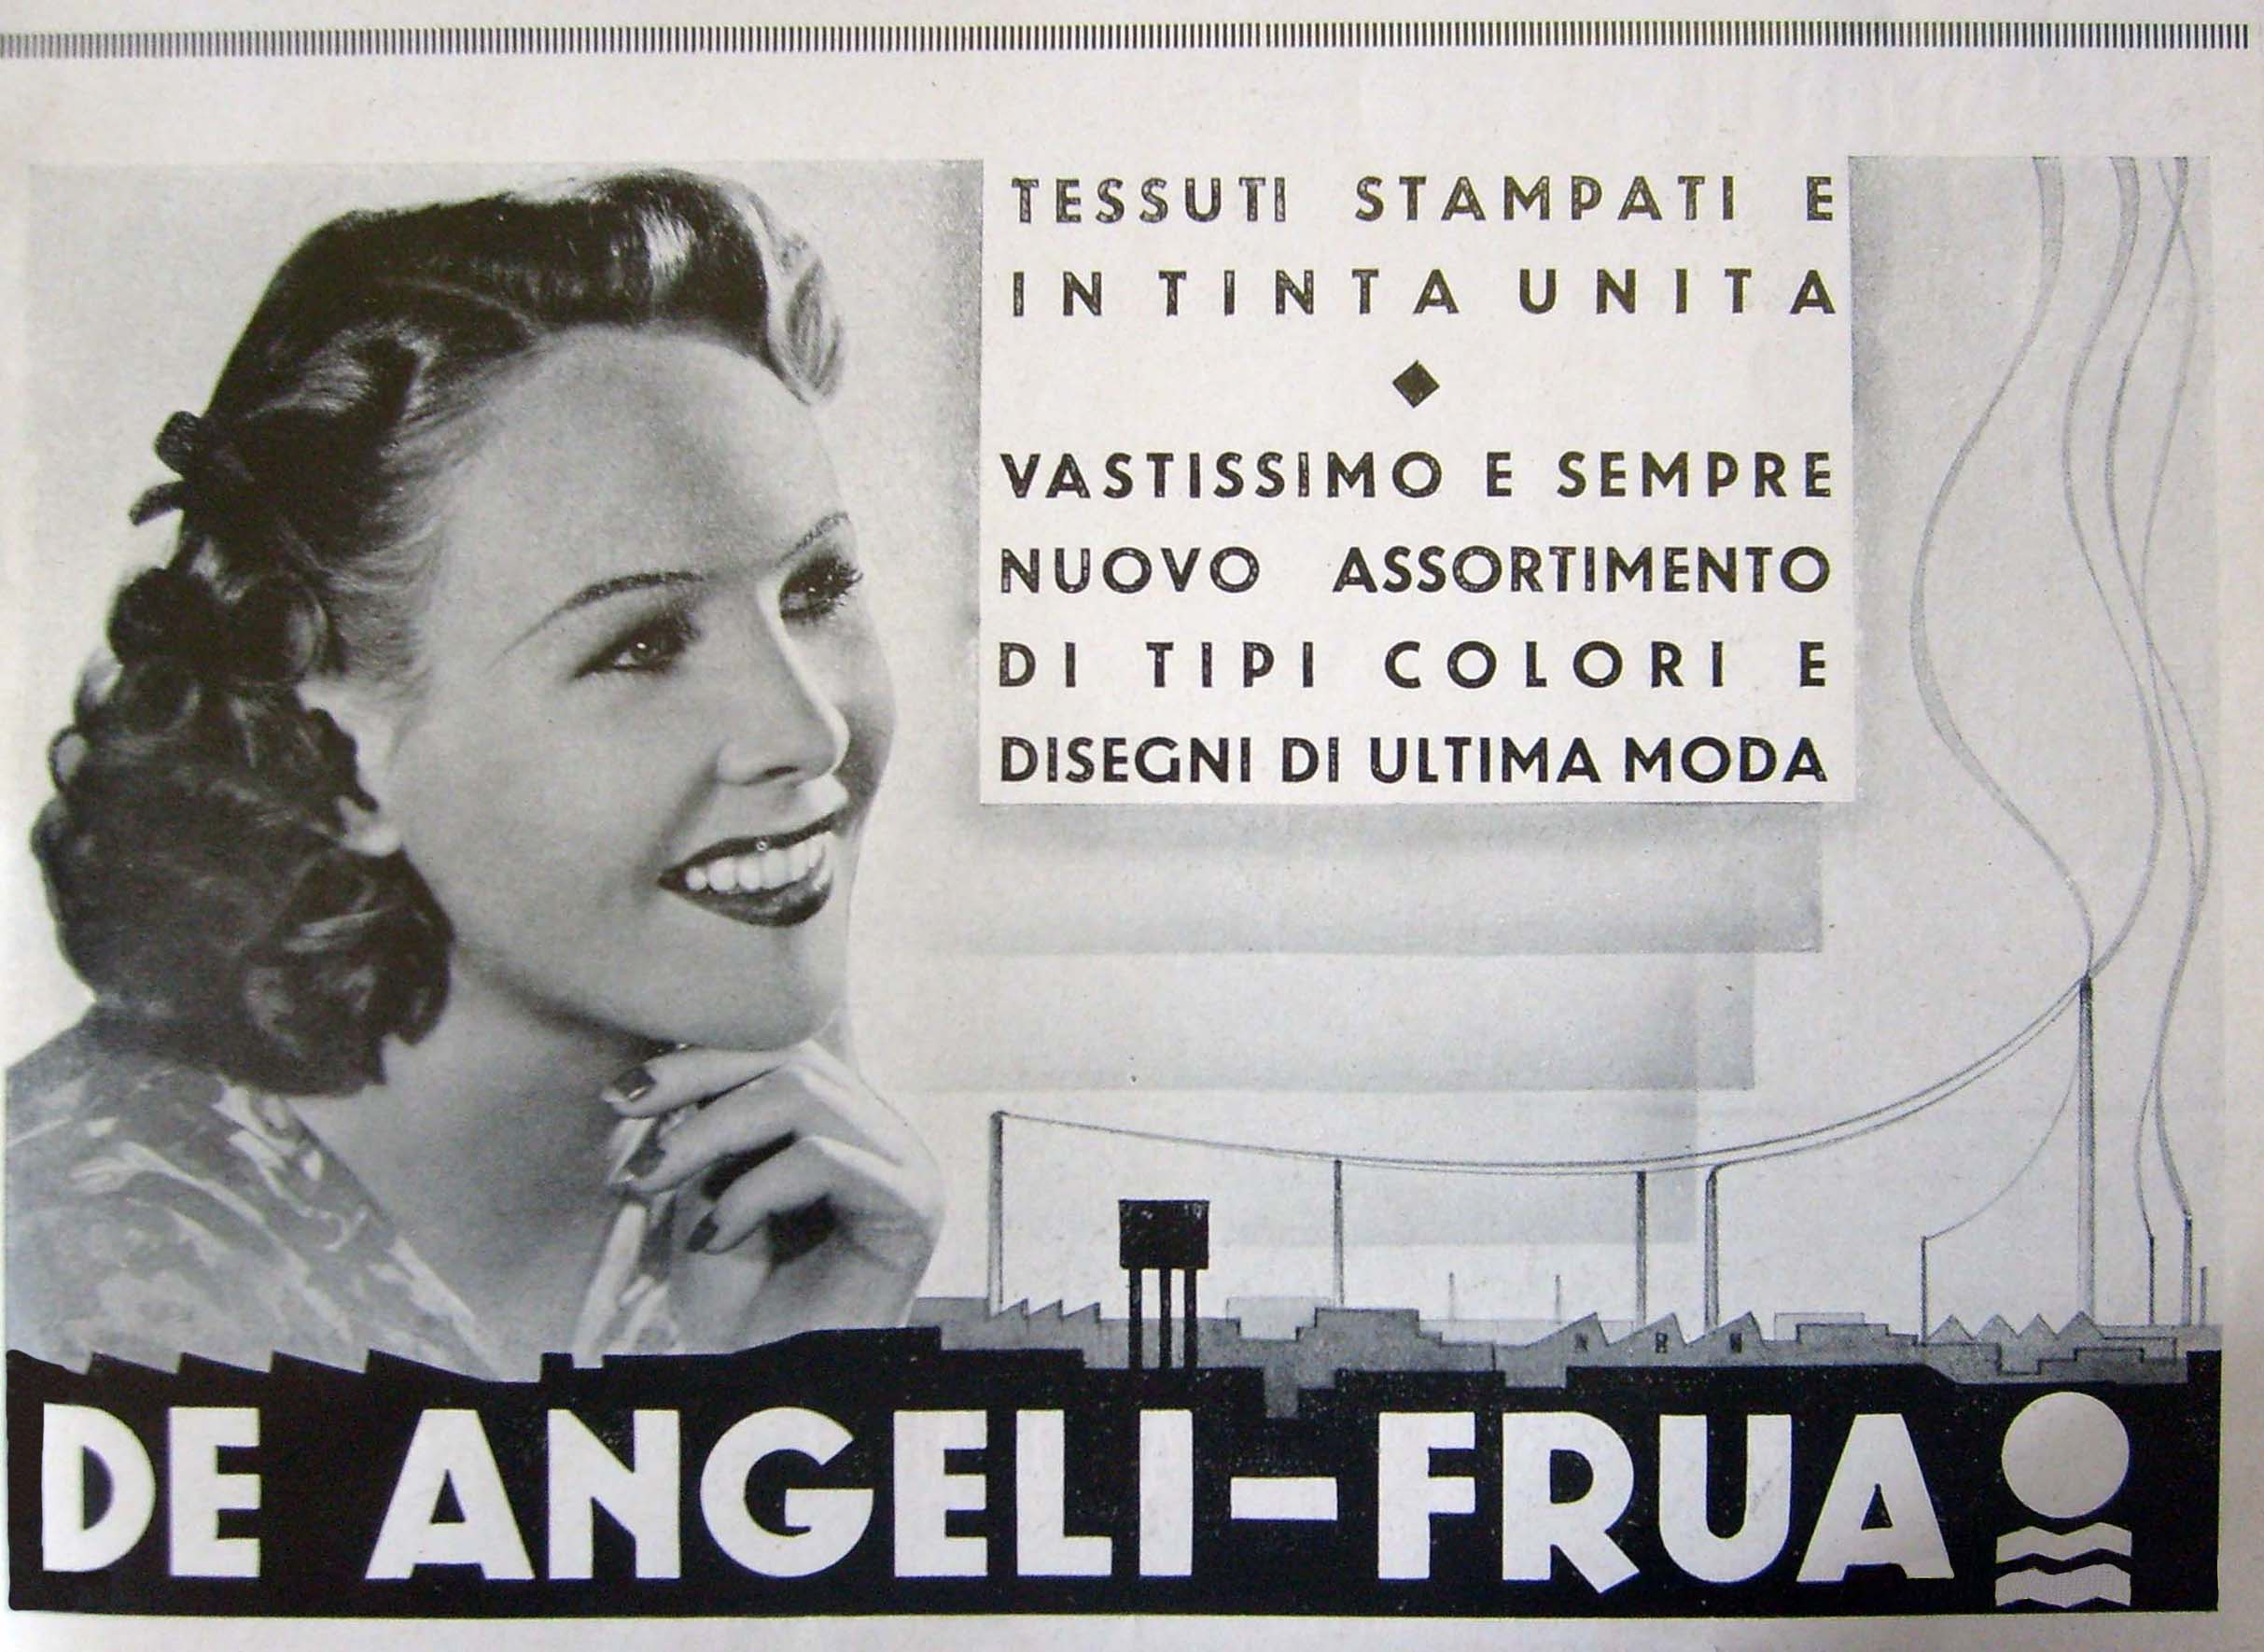
\includegraphics[width=\textwidth]{deangeli_2.jpg}
	\caption{}
	\label{fig:deangeli_2}
\end{figure}
\begin{figure}[h]
	\centering
		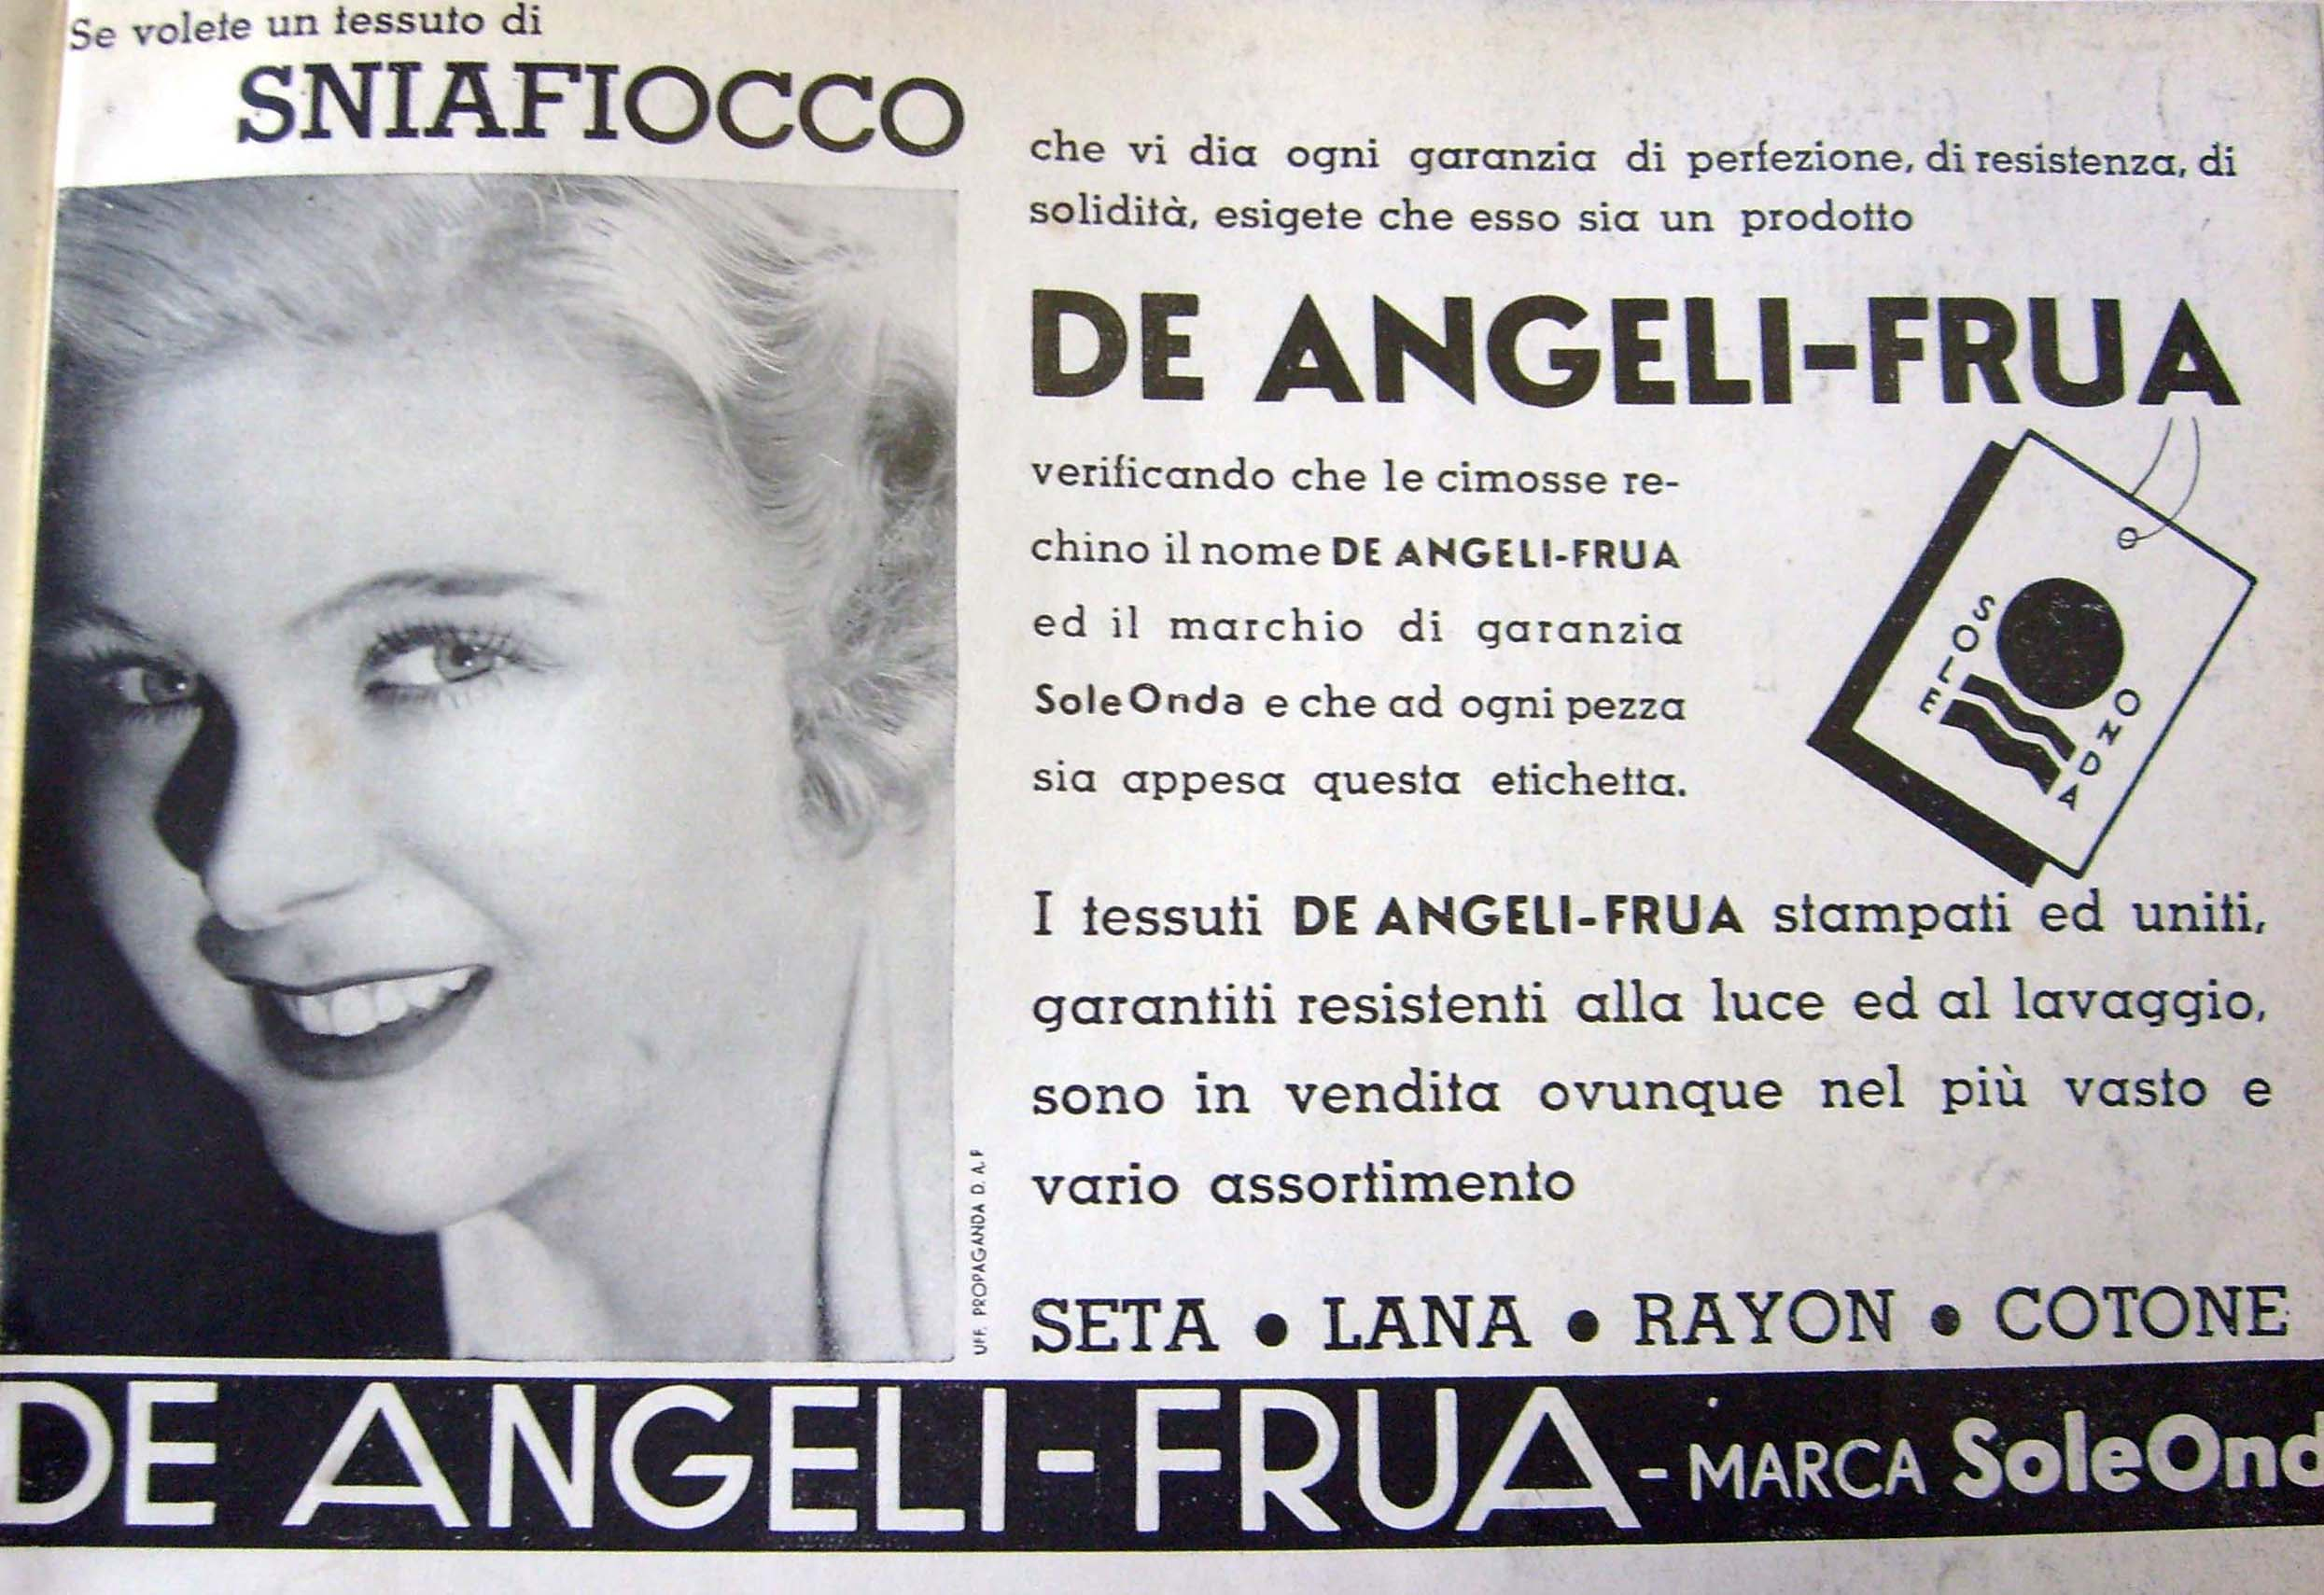
\includegraphics[width=\textwidth]{deangeli_3.jpg}
	\caption{}
	\label{fig:deangeli_3}
\end{figure}


\clearpage
